\section{Fundamental Observations}

\begin{frame}{Fundamental Observations}{Sky is Dark}
	Heinrich Olber came up with the observation that
	the Sky is dark, when it really shouldn't be. If we assume universe
	to be infinitely long, and indefinitely long, then using calculated
	parameters like $n$ (number density of stars), $L_*$ luminosity of
	an average star, Radius of star $R_*$, etc, we can see that luminosity of night sky far outweighs the
	luminosity of night sky by 10 trillion.

	Start with the fact that we need only one start with $R_*$ to block
	our view to the rest of the stars behind it. Say this star is at
	distance $\lambda$
	$$ 1 = n V $$
	$$ 1 = n \pi r^2 \lambda $$
\end{frame}

\begin{frame}{Fundamental Observations}{Sky is Dark}
This is called Olber's paradox and there are various explanations to this
effect:
\begin{itemize}[<+->]
	\item \textbf{The space is not transparent and there are particles that absorb
		light.} This can't be true because any body that absorbs light
		will eventually start emitting light like BBR.
	\item \textbf{Assumption that Universe is infinitely large is wrong.}
	\item \textbf{Assumption that Universe has existed forever is wrong.}:
		This supports to a big bang model, rather than a steady state one.
	\item \textbf{If universe were to be constantly expand, then the
		brightness of the light source would decrease as it reaches us.}
		This doesn't explain why we don't see stars in all directions
		though.
\end{itemize}
\end{frame}


\begin{frame}{Fundamental Observations}{Universe is Isotropic and Homogenous}

In small scales its not. In the orders of 100 Mpc though we can consider
universe to be both "Isotropic" and "Homogenous"


\includegraphics[width=4in]{1}

\end{frame}

\begin{frame}{Fundamental Observations}{Early Observations}
    Early astronomers and philosophers like Galileo and Coppernicus disproved the
    geocentric model and adopted the heliocentric one. But according to
    Coppernicus, even the heliocentric model doesn't explain the speciality of
    our place.

    This leads us to the Coppernican principle that when built on top of it
    leads us to the Cosmological principle.

    "There is nothing special or privileged about our location in the
    universe." - Coppernicus

    "We're not only not number one, but we are next to none" - Cosmological
    Principle.
\end{frame}


\begin{frame}{Fundamental Observations}{Redshift is proportial to Distance}

Redshift is caused due to Doppler's effect in EM waves which cause a shift in
the emitted wavelength versus the observed
$$ \frac{v}{c} \approx z = \frac{\lambda_{ob} - \lambda_{em}}{\lambda_{em}} $$
We can use the doppler shift to explain that, objects which move farther away
produce a red shift and the ones, coming closer cause blue shift.

Scientists like Lemaitre, observed that 37 of 42 observed objects were
redshifted rather than blueshifted. Hubble was another scientists who calculated
that there is a linear relation between the redshifts (z) and the distances of
the objects from Earth.

$$ z = \frac{H_0}{c} r $$

Using $ \frac{v}{c} \approx z $, we get
$$ v = H_0r  $$


\end{frame}

\begin{frame}
 Does this mean that all particles are moving
away from us? That would violate the cosmological principle.

\begin{columns}
	\column{.5\textwidth}
	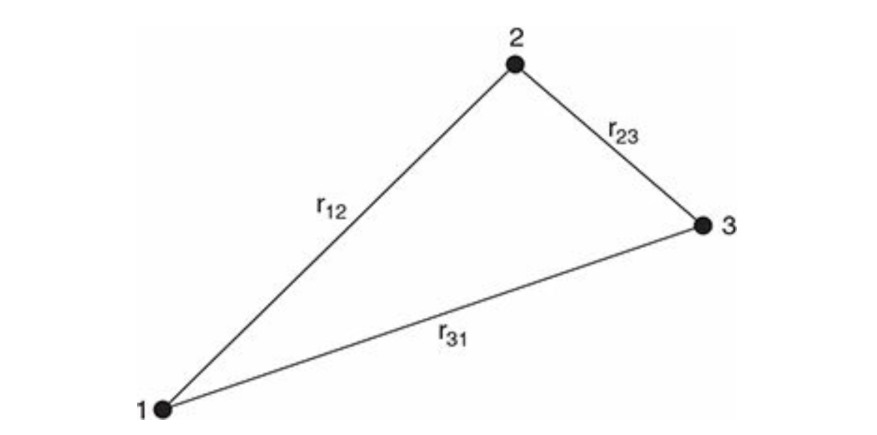
\includegraphics[width=\textwidth]{2}
	\column{.5\textwidth}
	$$ r_{12} = a(t)r_{12}(t_0) $$
	$$ v_{12} = \frac{dr_{12}}{dt} = \dot a(t)r_{12}(t_0) = \frac{\dot a}{a}
	r_{12}(t)$$
	Thus,
	$$ \frac{v_{12}(t)}{r_{12}(t)} = \frac{\dot a}{ a } = H_0 $$

\end{columns}

\vspace{1cm}

This means the universe has expanded in linear fashion. Thus we can
estimate the lifetime of universe by $t = \frac{r}{v} = H_0^{-1}$ of any object.
This is a good estimated of the lifetime of universe, $t_0 = 14.38 Gyr$.

\end{frame}

\begin{frame}{Fundamental Observations}{Different Types of Particles}
    I will cover only photon and neutrino.

    \begin{itemize}[<+->]
	    \item \textbf{Neutrino:}
		    This is mostly a relativistic particle but has rest mass
		    energy of about $10^{-2} eV$. There are three types of
		    neutrinos, and each of these type have three mass states
		    $(m_1, m_2, m_3)$. Due to quantum occilations the rest
		    energy keeps changing and this  energy can be calculated.
		    $$ (m_2^2 - m_1^2)c^4 \approx 7.5 \times 10^{-5} $$
		    $$ (m_3^2 - m_2^2)c^4 \approx 2.4 \times 10^{-3} $$
	    But this doesn't give us an estimate of individual mass states.
	    Approximations can be made by calculating  the rest energy of
	    sum of $(m_e + m_t + m_u) = (m_1 + m_2 + m_3)$, which comes out to
	    be between $(0.057, 0.3) eV$.
    \end{itemize}
    $$  $$

\end{frame}

\begin{frame}
	\begin{itemize}[<+->]
	    \item \textbf{Photon:}
		    Even though they have no mass, they do have energy density
		    which can be calculated using the blackbody function:
		    $$ \epsilon(f)df = \frac{8\pi h}{c^3} \frac{f^3 df}{
		    e^{\frac{hf}{kT}} - 1 } $$

		    We can use it to calculate the energy and the number density
		    by integrating over all frequencies.
		    $$ \epsilon_\gamma = \alpha T^4 $$
		    Where $\alpha = \frac{\pi^2}{15} \frac{k^4}{\hbar^3 c^3}$,
		    $$ n_\gamma = \beta T^3 $$
		    Where $\beta = \frac{2.4041}{\pi^2} \frac{k^3}{\hbar^3 c^3}$,

		    One great thing about radiation is that we can calculate the
		    temperature corresponding to a give frequency using
		    $$ E_{mean} = h f_{mean} = 2.7 k T  $$
		  \end{itemize}
\end{frame}

\begin{frame}{Fundamental Observations}{Comsological Microwave Background}
There have been other models being proposed too which go against the fact that
universe is expanding linearly, one such is Steady State model.
$$ \frac{dr}{dt} = H_0 r $$
$$ r = e^{H_0 t}$$
Another postulate of this model is that the Mass density of the universe is
constant. But if universe is expanding and density is constant, that would mean
new matter is being produced, but that violates various laws of physics.

But this model got disproved once the CMB waves were discovered and it gave an
accurate representation


\end{frame}

\begin{frame}
	It was observed that there is an isotropic background of microvawe
	radiation all over the universe and the wavelength of this corresponds to
	that of microwaves, thus temperature can be calculated by above relation
	as $T_0 = 2.7255 K$. This can be again used to calculate the energy
	density and the number density as.
	$$ \epsilon_\gamma = 4.175 \times 10^{-14} MeV/m^3
	, n_\gamma = 4.107 \times 10^8 m^{-3} $$

	It is said that CMB is a relic to the past when the radiation was so
	dominant, that it used to render the universe opaque and matter was
	ionized. Then this energy density fell off to a point where the energy
	of these photons couldn't photoionize matter anymore.

	We can start with the second law of thermodynamics and actually
	calculate the dependence of temperature of CMB to the expansion
	coefficient
	$$ dQ = dE + PdV $$
\end{frame}
